\let\negmedspace\undefined
\let\negthickspace\undefined
\documentclass[journal]{IEEEtran}
\usepackage[a5paper, margin=10mm, onecolumn]{geometry}
%\usepackage{lmodern} % Ensure lmodern is loaded for pdflatex
\usepackage{tfrupee} % Include tfrupee package

\setlength{\headheight}{1cm} % Set the height of the header box
\setlength{\headsep}{0mm}     % Set the distance between the header box and the top of the text

\usepackage{gvv-book}
\usepackage{gvv}
\usepackage{cite}
\usepackage{amsmath,amssymb,amsfonts,amsthm}
\usepackage{algorithmic}
\usepackage{graphicx}
\usepackage{textcomp}
\usepackage{xcolor}
\usepackage{txfonts}
\usepackage{listings}
\usepackage{enumitem}
\usepackage{mathtools}
\usepackage{gensymb}
\usepackage{comment}
\usepackage[breaklinks=true]{hyperref}
\usepackage{tkz-euclide} 
\usepackage{listings}
% \usepackage{gvv}                               

\def\inputGnumericTable{}                      
\usepackage[latin1]{inputenc}                    
\usepackage{color}                              
\usepackage{array}                             
\usepackage{longtable}                          
\usepackage{calc}                               
\usepackage{multirow}                           
\usepackage{hhline}                            
\usepackage{ifthen}                          
\usepackage{lscape}
\begin{document}

\bibliographystyle{IEEEtran}
\vspace{3cm}

\title{2.2.17}
\author{AI25BTECH11024 - Pratyush Panda
}
\maketitle
% \newpage
% \bigskip
{\let\newpage\relax\maketitle}

\renewcommand{\thefigure}{\theenumi}
\renewcommand{\thetable}{\theenumi}
\setlength{\intextsep}{10pt} % Space between text and floats


\numberwithin{equation}{enumi}
\numberwithin{figure}{enumi}
\renewcommand{\thetable}{\theenumi}

\textbf{Question: } \\
Find the angle between the lines: \\
\begin{align}
y=\brak{2-\sqrt{3}}\brak{x+5} \, \text{and}
\end{align}

\begin{align}
y=\brak{2+\sqrt{3}}\brak{x-7}.
\end{align}

\textbf{Solution: } \\
The given equations can be written as;
\begin{align}
\brak{2-\sqrt{3}}x - y = \brak{\sqrt{3}-2}5
\end{align}
\begin{align}
\brak{2+\sqrt{3}}x - y = \brak{2+\sqrt{3}}7
\end{align}

From this, we can see that the normal vectors of the lines can  be expressed as,

\begin{align}
\Vec{n_1}=\myvec{2-\sqrt{3} \\ -1}, \Vec{n_2}=\myvec{2+\sqrt{3} \\ -1}
\end{align}


The angle between the lines can be obtained as;

\begin{align}
\cos{\theta}=\frac{n_1^Tn_2}{||n_1||\,||n_2||}=\frac{1}{2}
\end{align}
\begin{align}
or, \, \theta=60^\circ
\end{align}

\begin{figure}[H]
\centering
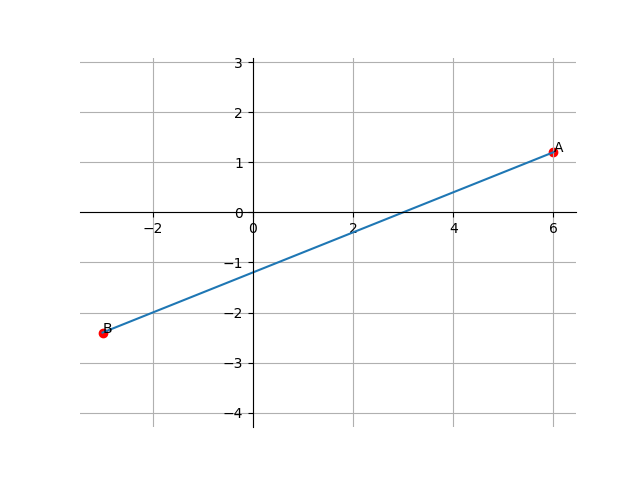
\includegraphics[width=0.6\columnwidth]{figs/img.png}
\caption*{}
\end{figure}

\end{document}
